\documentclass{article}

\usepackage{tikz}
\usepackage{graphicx}
\usepackage{listings}
\usepackage{float}
\usepackage{setspace}
\usepackage{subcaption}
\usepackage[bottom]{footmisc}

\title{Relazione prova finale Reti Logiche}
\date{09/03/2021}
\author{Vlad Cimpeanu: 10606922\\ Danilo Castiglia: 10685118}

\begin{document}

\maketitle
\pagenumbering{gobble}

\pagenumbering{arabic}
%\setlength{\parskip}{3em} %added in Vlad's version

\begin{figure}[h!] %%%%     H al posto di h! se dà problemi      %%%%%
\centering
  \includegraphics[scale = 0.2]{polimi}
  \label{fig:polimi}
\end{figure}

\newpage

\section{Introduzione}
%Insieme
Lo scopo di questo progetto è di programmare una FPGA al fine di equalizzare delle immagini date in ingresso. Queste ultime sono memorizzate in una memoria ram di tipo sincrono.\\
Le immagini sono in scala di grigi e ogni pixel assume valori da 0 a 255, dove 0 corrisponde al colore nero e 255 al colore bianco. La dimensione massima di ciascuna immagine è di 128 pixel in larghezza e 128 pixel in altezza, per un peso totale di 16KB.\\
Il modulo progettato, si aspetta di trovare in memoria nei primi due indirizzi la dimensione rispettivamente di larghezza e altezza, seguite da tutti i pixel dell'immagine, riga per riga. Data l'immagine in ingresso, il componente effettua alcune semplici operazioni e restituisce l'immagine aumentandone il contrasto. La tecnica che viene utilizzata è l'\textbf{equalizzazione dell'istogramma}, che consiste nello spalmare i valori di intensità dell'immagine su tutto l'intervallo  (da 0 a 255).\\

\begin{figure}[h!]
  \centering
  \begin{subfigure}[b]{0.4\linewidth}
    \includegraphics[width=\linewidth]{pre}
    \caption{Pre}
  \end{subfigure}
  \begin{subfigure}[b]{0.4\linewidth}
    \includegraphics[width=\linewidth]{post}
    \caption{Post}
  \end{subfigure}
  \caption{The same image. Pre e post.}
  \label{fig:coffee}
\end{figure}


\section{Architettura}
\subsection{Scelte progettuali}
%Insieme
Per la realizzazione di questo progetto si è deciso di dividere \textbf{unità di elaborazione} e \textbf{unità di controllo}, facendo uso di un datapath e di una macchina a stati di Moore. Il datapath utilizza una rete combinatoria per il calcolo dei logaritmi, sommatori, sottrattori, comparatori, multiplexer e registri, con lo scopo di elaborare tutti i calcoli richiesti dalla macchina a stati.

\subsection{Datapath}
%Vlad: Row, Column, Address
%Danilo: New_pixel, Max/Min: init ti permette di resettare il valore
\paragraph{Row \& Column counter\\}

Il modulo Row \& Column counter è stato ideato con lo scopo di riconoscere la fine dell'immagine da leggere che si trova memorizzata all'interno della RAM.\\
Memorizzando le dimensioni di larghezza e altezza nei rispettivi registri e utilizzando dei contatori che tengono traccia delle righe e delle colonne per riga già lette è possibile parallelizzare la ricerca della fine dell'immagine con la lettura della stessa.\\
Così facendo si va a ricreare quello che in programmazione è definito come nested loop:

\begin{lstlisting}[language=Python, caption={Nested loop in pseudocodice.},captionpos=b]
address = 2
for column in range(column_max):
    for row in range(row_max):
        address += 1
\end{lstlisting}

La scelta di adottare questa tecnica è stata dettata dall'intenzione di voler modellare un circuito efficiente. Nel caso in cui si fosse deciso di seguire una via più semplice, ovvero l'utilizzo di un moltiplicatore, si sarebbe ottenuto un aumento significativo del critical path diventando un collo di bottiglia per l'intero circuito.\\
È interessante notare come all'aumentare delle dimensioni dell'immagine è inevitabile che il numero di istruzioni da eseguire sia maggiore: con l'utilizzo di un moltiplicatore si andrebbe inoltre, ad incrementare la durata del clock compromettendo la velocità del circuito, mentre con questo modulo il clock rimane inalterato.\\
Per migliorare l'efficienza del componente, si è scelto di verificare che le dimensioni dell'immagine da caricare siano diverse da 0 e in caso contrario di segnalare questa anomalia alla FSM che in seguito gestirà in maniera appropriata tale situazione. L'assenza dei comparatori (utilizzati a tale scopo) non preclude il funzionamento corretto del circuito, tuttavia nel caso pessimo si effettuano più di 2\textsuperscript{16} operazioni elementari inutili.

\begin{figure}[h!]
\centering
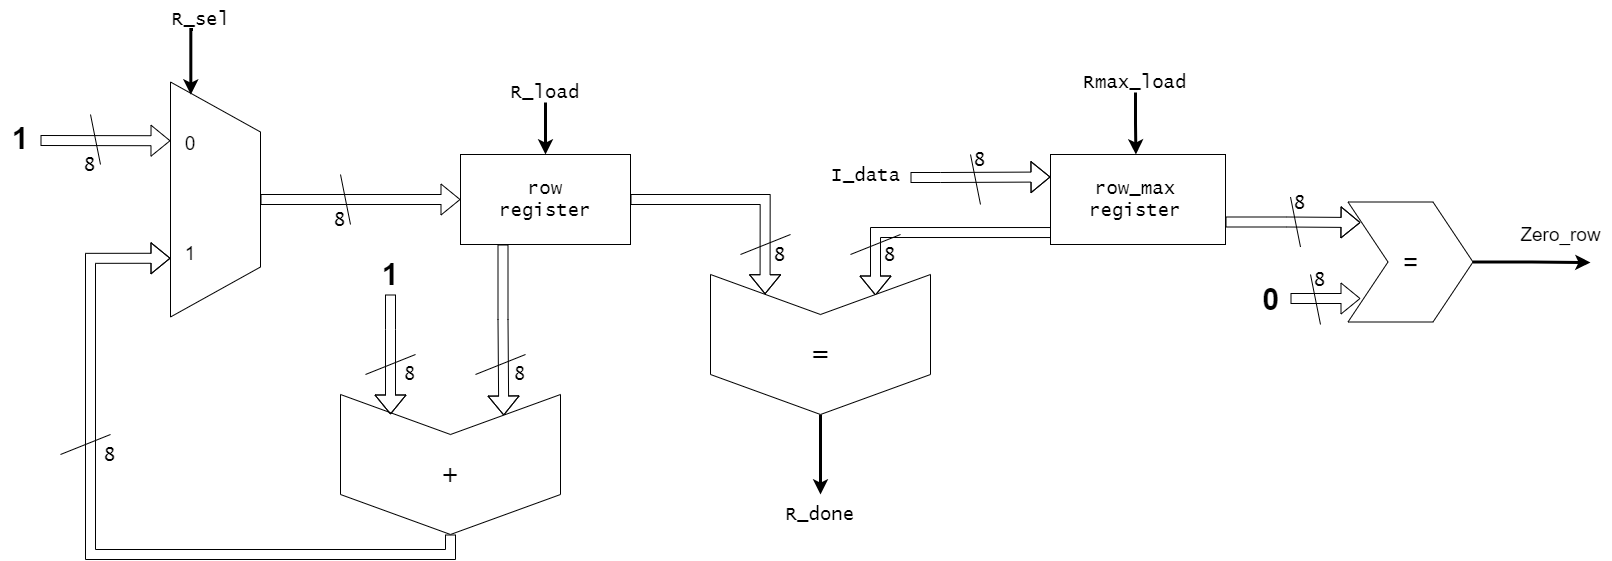
\includegraphics[scale=0.2]{row_counter.png}%######ROWS_COUNTER.PNG NEEDED IN THE SAME DIRECTORY TO WORK PROPERLY
\caption{Rappresentazione schematica del contatore di righe.}
\end{figure}
\begin{figure}[h!]
\centering
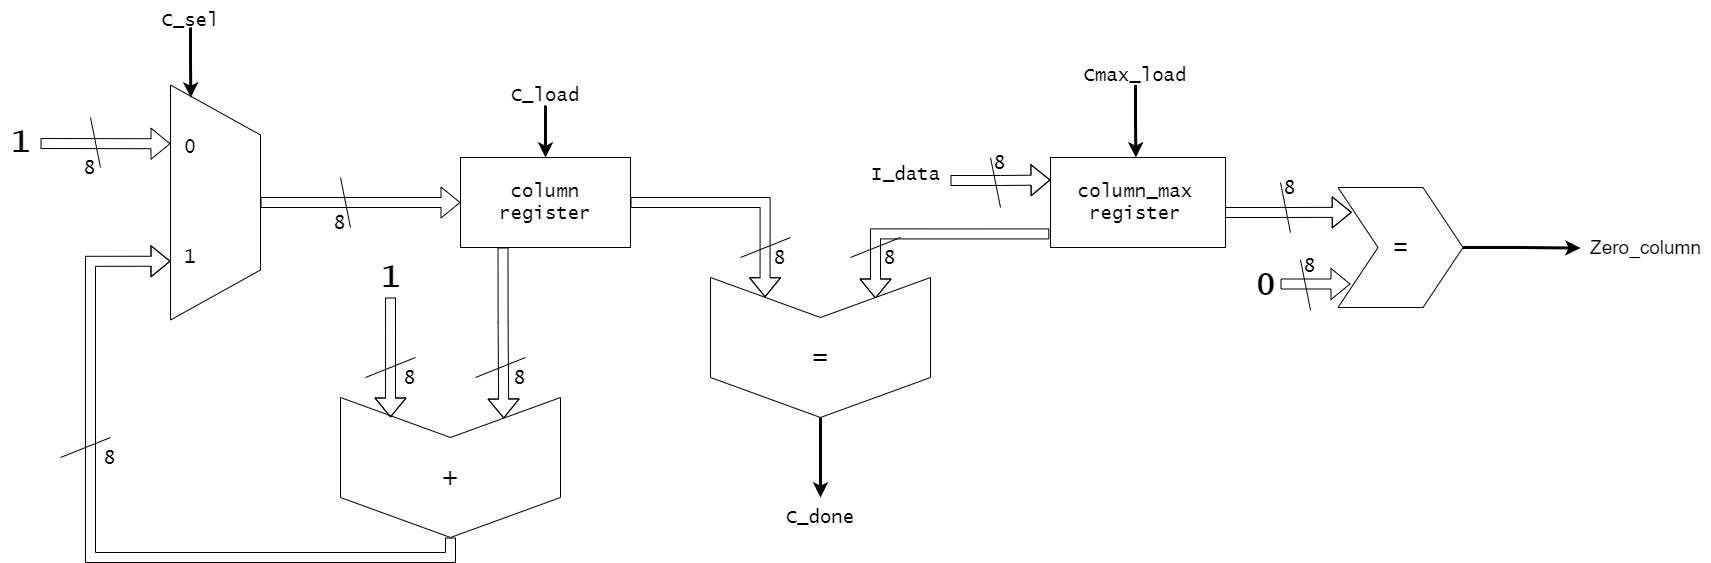
\includegraphics[scale=0.2]{column_counter.png} %######COLUMNS_COUNTER.PNG NEEDED IN THE SAME DIRECTORY TO WORK PROPERLY
\caption{Rappresentazione schematica del contatore di colonne.}
\end{figure}

\paragraph{Address Counter\\}

Il modulo Address Counter è stato sviluppato per richiedere gli indirizzi alla RAM, sia in fase di lettura che in fase di scrittura.\\
Come si può notare dalla Figure 3 il modulo è principalmente formato da due contatori e da un multiplexer a 4 ingressi. Il multiplexer seleziona quale valore dell'indirizzo o\_address debba essere mandato in uscita:
\begin{itemize}
    \item l'ingresso 0 restituisce il valore salvato nell'address register;
    \item l'ingresso 1 restituisce il valore salvato nell'address2 register;
    \item l'ingresso 2 restituisce l'indirizzo 0x00, utilizzato per richiedere la larghezza dell'immagine;
    \item l'ingresso 3 restituisce l'indirizzo 0x01, utilizzato per richiedere l'altezza dell'immagine.
\end{itemize}
In fase di lettura viene utilizzato solo address register dove viene memorizzato l'indirizzo del prossimo pixel da leggere, mentre nella fase di scrittura viene sfruttato anche address2 register.\\
Al termine della fase di lettura, address register contiene già il primo indirizzo dove scrivere il nuovo pixel, mentre address2 register viene inizializzato al valore dell'indirizzo contenente il primo pixel originale, infine viene salvato il valore di address register in un nuovo registro chiamato 'end register'.
Durante la fase di scrittura i valori di address register e address2 register vengono incrementati in parallelo fino a quando address2 register contiene lo stesso valore di end register, in quanto esso indica che tutti i pixel originali sono già stati letti e quindi trasformati.

\begin{figure}[h!]
\centering
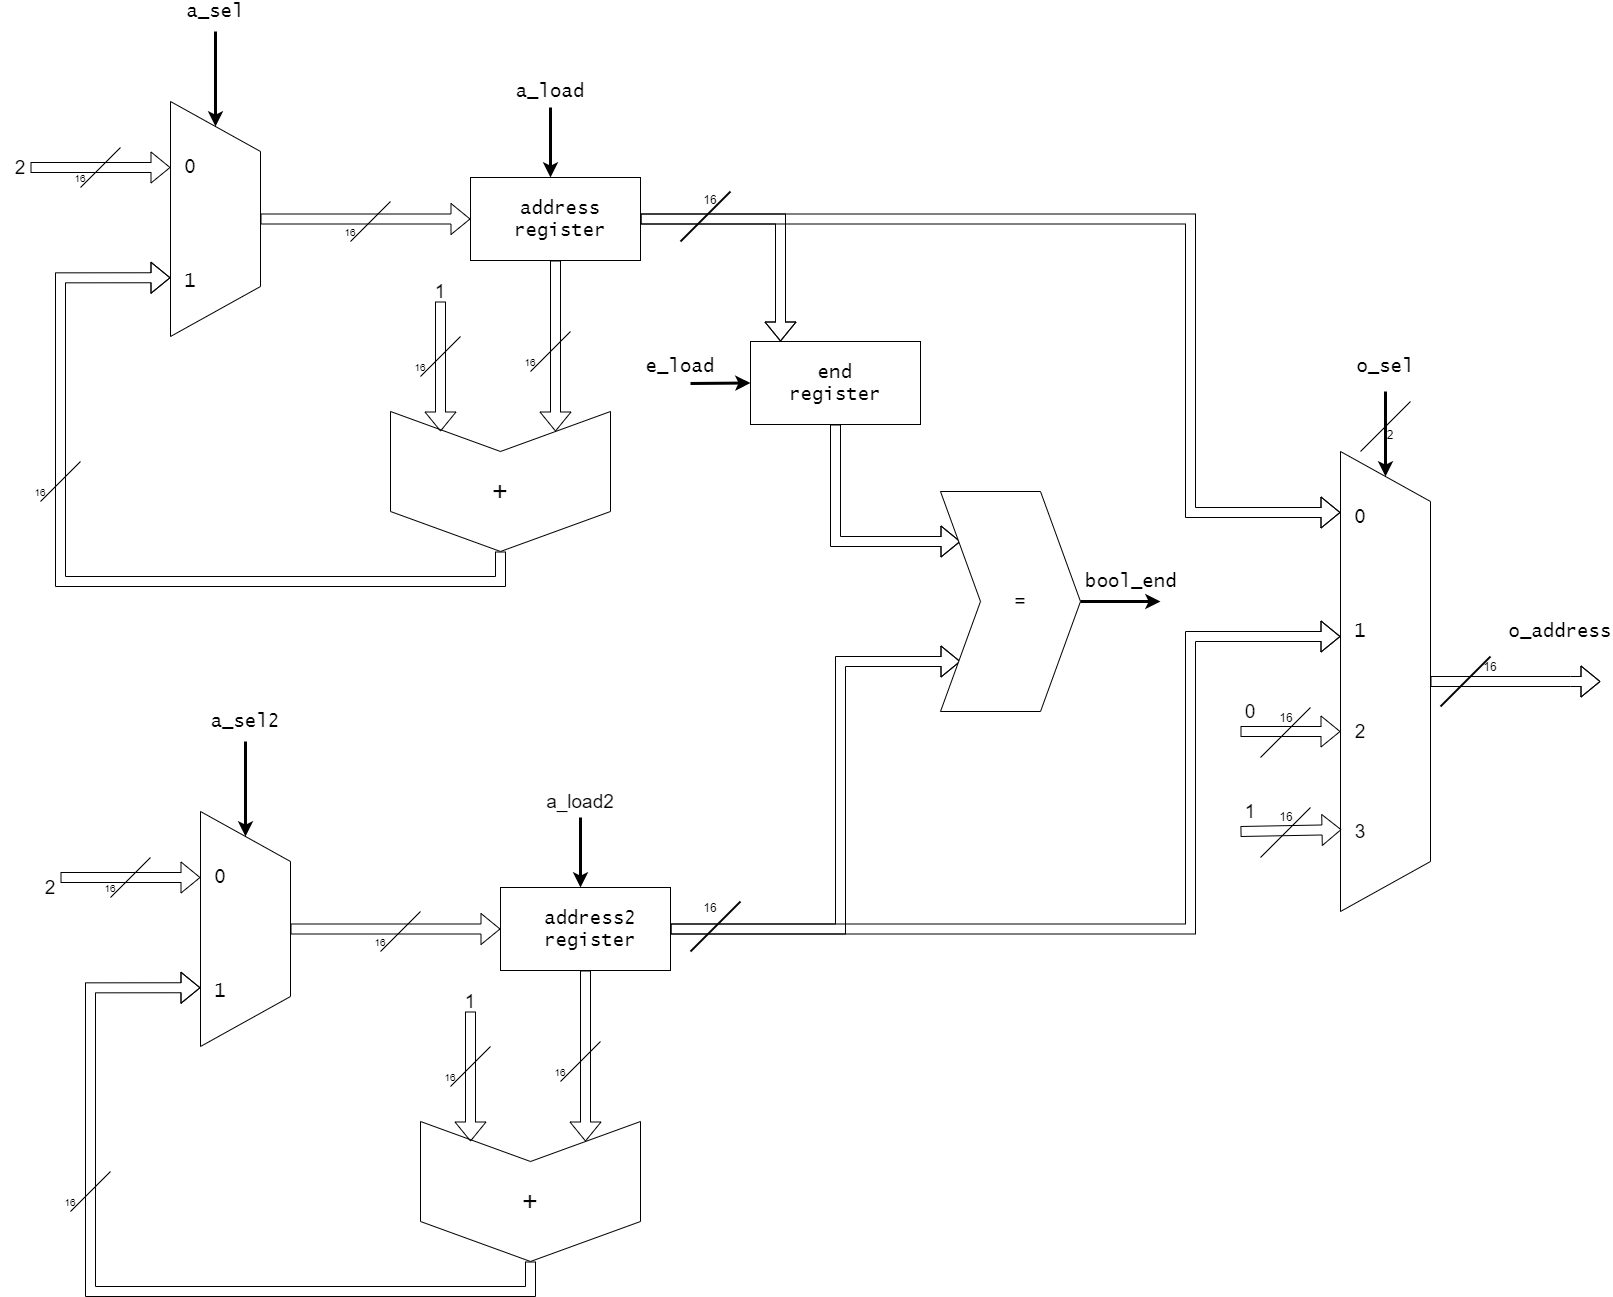
\includegraphics[scale=0.2]{final_address_calculator_module.png}%######final_address_calculator_module.PNG NEEDED IN THE SAME DIRECTORY TO WORK PROPERLY
\caption{Rappresentazione schematica dell'Address Counter.}
\end{figure}


\paragraph{Max \& Min calculator\\}

Questo modulo permette di trovare i valori massimo e minimo dei pixel presenti nell'immagine.\\
Il funzionamento del modulo è semplice. Vengono impiegati due registri: max register e min register, nei quali alla fine del calcolo saranno presenti rispettivamente il valore massimo e minimo dei pixel dell'immagine.\\
Inizialmente,(con l'ausilio del segnale "init") viene caricato in max register e min register il valore del primo pixel dell'immagine. Successivamente, per ogni altro pixel dell'immagine, lo si confronta con i valori contenuti nel registro max e min e, se il valore del pixel è maggiore del massimo (contenuto in max) o minore del minimo (contenuto in min), si aggiornano i valori nei due registri.\\
Il calcolo termina dopo aver letto e processato l'ultimo pixel dell'immagine.

\begin{figure}[h!] %%%%     H al posto di h! se dà problemi      %%%%%
  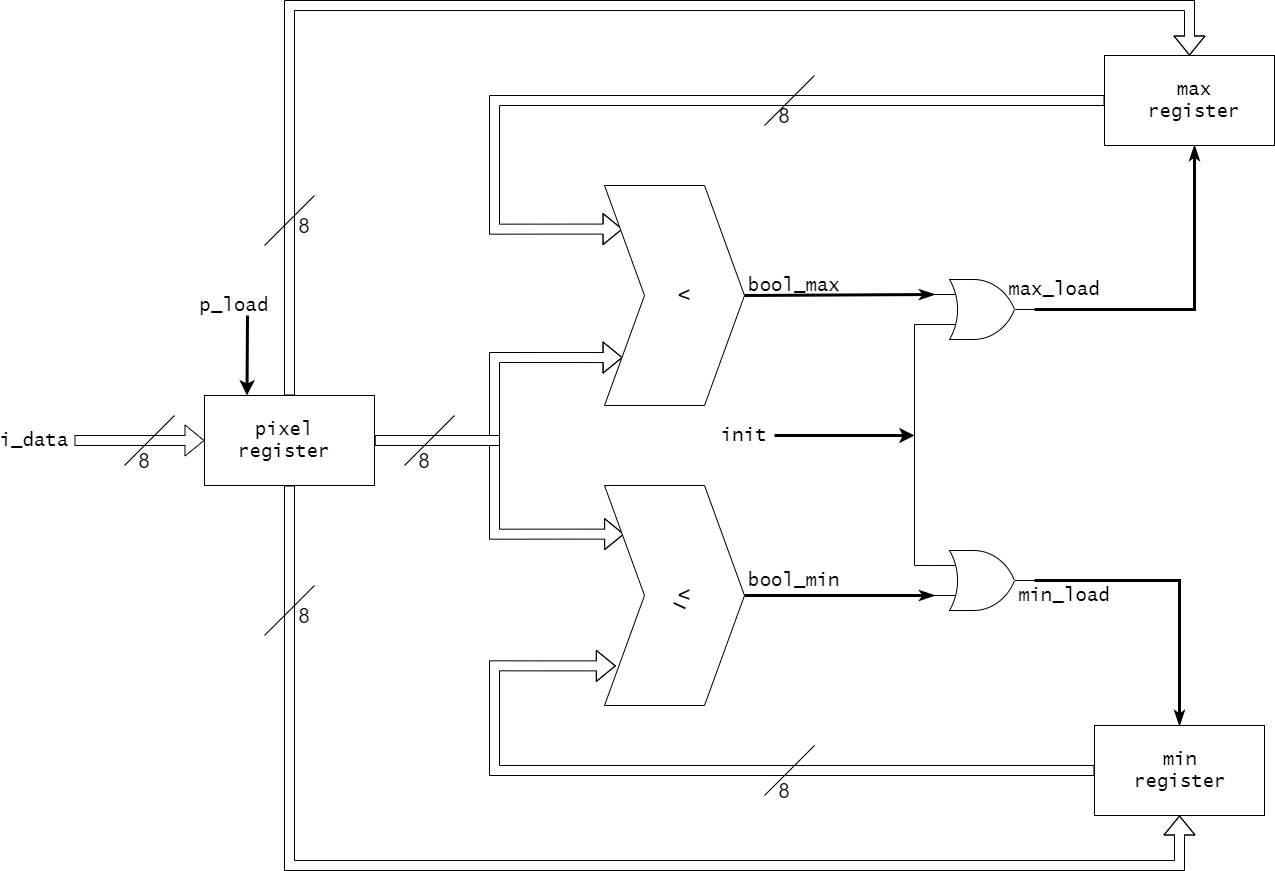
\includegraphics[width=\linewidth]{max_min_module}
  \caption{Rappresentazione schematica del modulo Max \& Min.}
  \label{fig:maxMin}
\end{figure}

\paragraph{New pixel value\\}
Questo modulo è il cuore dell'algoritmo di equalizzazione di immagini, calcola le seguenti funzioni:
\doublespacing
\singlespacing
DELTA\_VALUE = MAX\_PIXEL\_VALUE – MIN\_PIXEL\_VALUE

SHIFT\_LEVEL = (8 – FLOOR(LOG2(DELTA\_VALUE +1)))

TEMP\_PIXEL = (CURRENT\_PIXEL\_VALUE - MIN\_PIXEL\_VALUE) \textless\textless SHIFT\_LEVEL

NEW\_PIXEL\_VALUE = MIN( 255 , TEMP\_PIXEL)
\doublespacing
\singlespacing
Si presti particolare attenzione al fatto che DELTA\_VALUE assume valori compresi tra 0 e 255, perciò bastano 8 bit per rappresentarlo. Al contrario, DELTA\_VALUE + 1 necessiterà di 9 bit per essere correttamente rappresentato.\\
L'uscita del logaritmo sarà di 4 bit, poichè i valori da rappresentare sono compresi tra 0 e 8.\\
La funzione FLOOR(LOG2()) è stata implementata in maniera combinatoria con controlli a soglia:

\begin{table}[h!]
\centering
\begin{tabular}{| c | c |} 
 \hline
 Intervallo & Logaritmo \\
  \hline
 $x \in [~;~]$ & $log_2(x)$ \\ [0.5ex] 
 \hline\hline
 $[1;1]$ & 0 \\ 
 $[2;3]$ & 1 \\
 $[4;7]$ & 2 \\ 
 $[8;15]$ & 3 \\
 $[16;31]$ & 4 \\
 $[32;63]$ & 5 \\
 $[64;127]$ & 6 \\
 $[128;255]$ & 7 \\
 $[256;256]$ & 8 \\ [1ex] 
 \hline
\end{tabular}
\caption{Logaritmo Combinatorio.}
\end{table}

\begin{figure}[h!] %%%%     H al posto di h! se dà problemi      %%%%%
  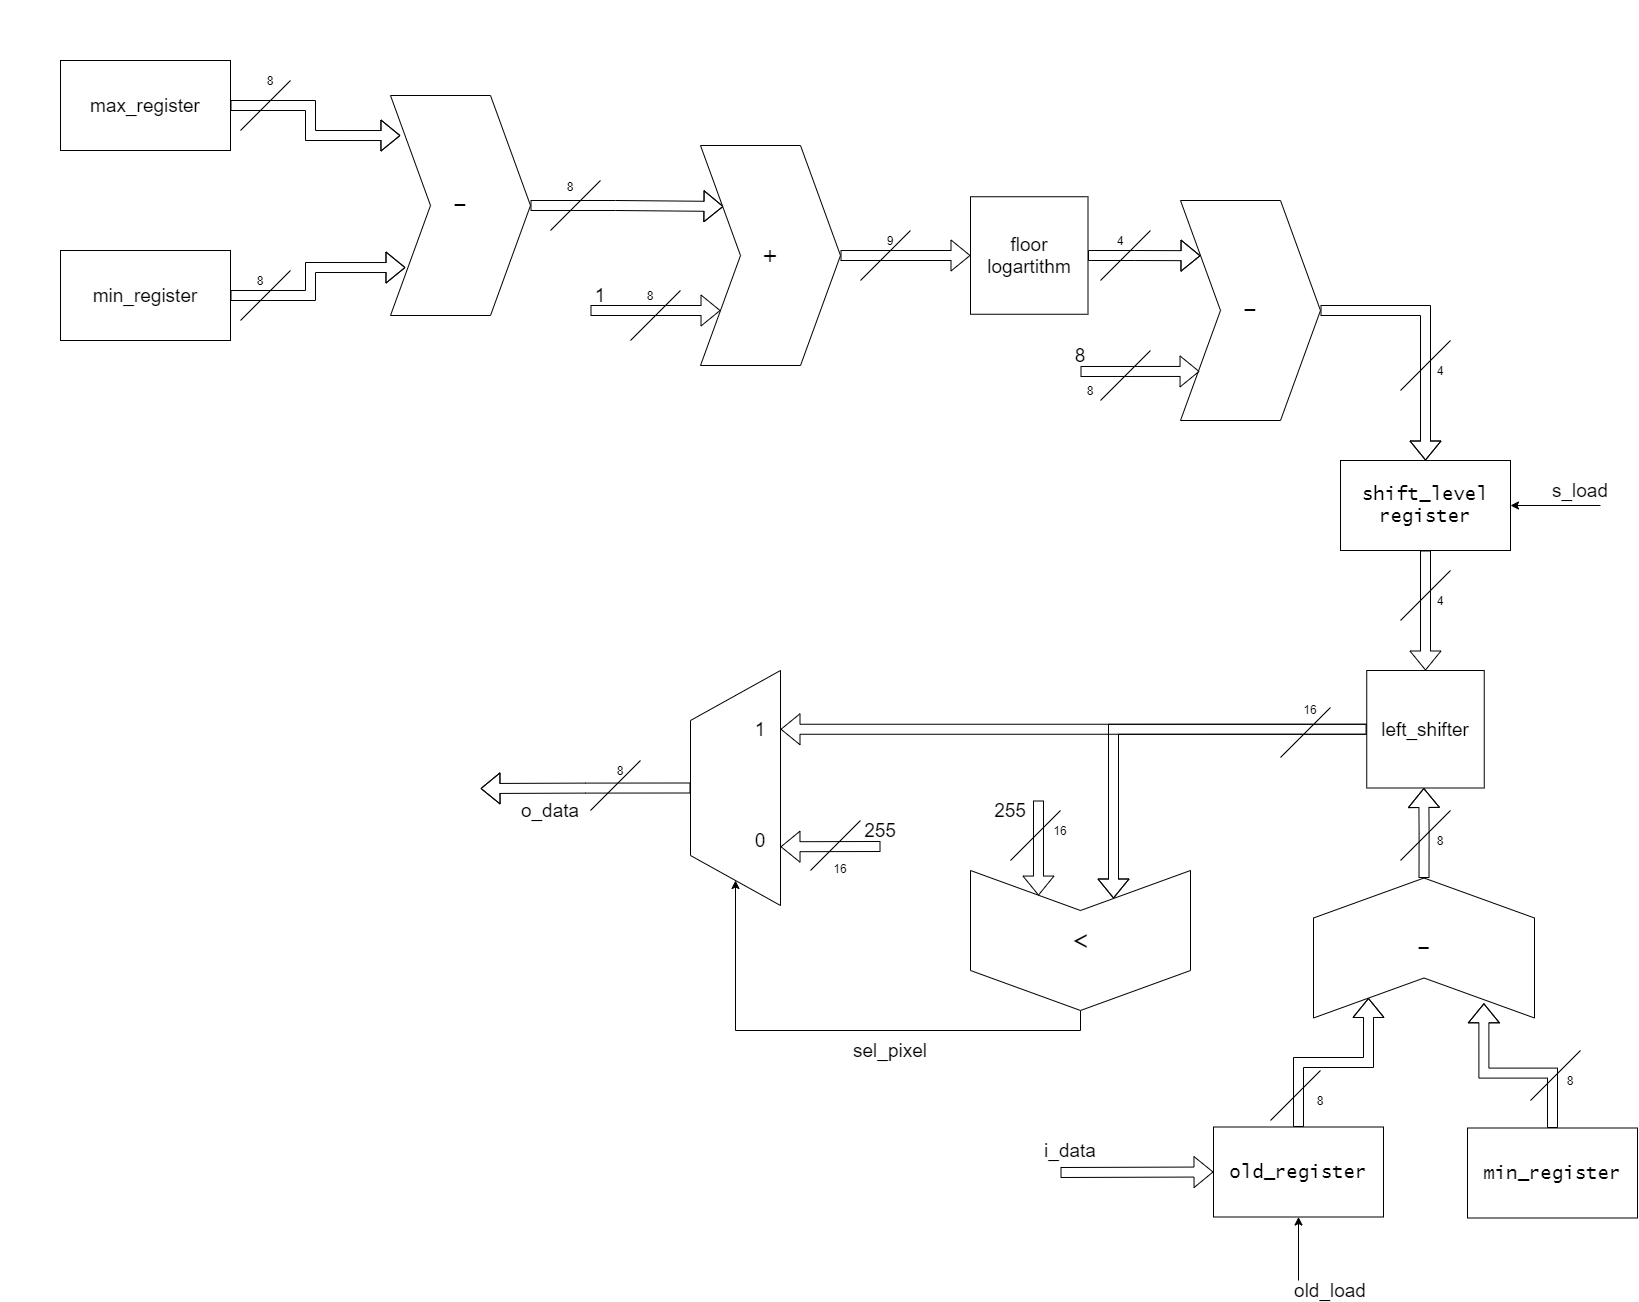
\includegraphics[width=\linewidth]{new_pixel_module}
  \caption{Rappresentazione schematica del modulo di calcolo funzioni.}
  \label{fig:newPixel}
\end{figure}

\subsection{Macchina a Stati}
%Vlad: S0...S8
%Danilo: S9...S14
\begin{center}
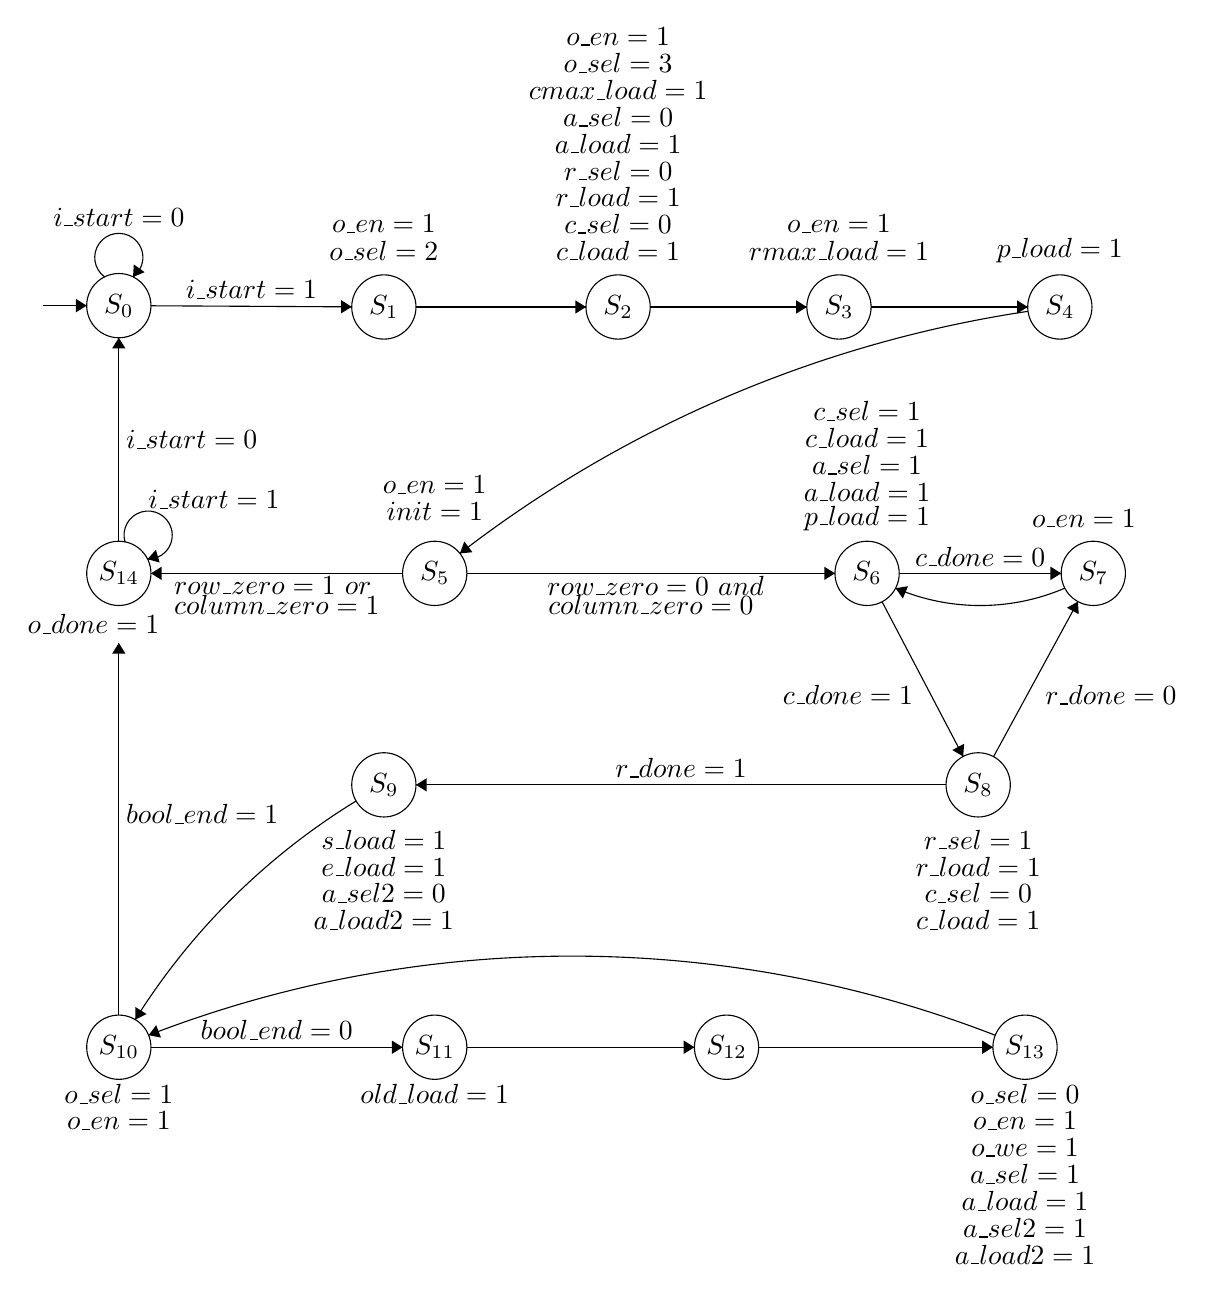
\begin{tikzpicture}[scale=0.17]
\tikzstyle{every node}+=[inner sep=0pt]
\draw [black] (5.9,-5.6) circle (2.4);
\draw (5.9,-5.6) node {$S_0$};
\draw [black] (25.7,-5.7) circle (2.4);
\draw (25.7,-5.7) node {$S_1$};
\draw [black] (43.2,-5.7) circle (2.4);
\draw (43.2,-5.7) node {$S_2$};
\draw [black] (59.7,-5.7) circle (2.4);
\draw (59.7,-5.7) node {$S_3$};
%S1
\draw (25.7,+0.5) node {$o\_en=1$};
\draw (25.7,-1.5) node {$o\_sel=2$};
%S2
\draw (43.2,+14.5) node {$o\_en=1$};
\draw (43.2,+12.5) node {$o\_sel=3$};
\draw (43.2,+10.5) node {$cmax\_load=1$};
\draw (43.2,+8.5) node {$a\_sel=0$};
\draw (43.2,+6.5) node {$a\_load=1$};
\draw (43.2,+4.5) node {$r\_sel=0$};
\draw (43.2,+2.5) node {$r\_load=1$};
\draw (43.2,+0.5) node {$c\_sel=0$};
\draw (43.2,-1.5) node {$c\_load=1$};
%S3
\draw (59.7,+0.5) node {$o\_en=1$};
\draw (59.7,-1.5) node {$rmax\_load=1$};
%S4
\draw (76.2,-1.5) node {$p\_load=1$};
%S5
\draw (29.5,-21) node {$init=1$};
\draw (29.5,-19) node {$o\_en=1$};
%S6
\draw (61.8,-13.5) node {$c\_sel=1$};
\draw (61.8,-15.5) node {$c\_load=1$};
\draw (61.8,-17.5) node {$a\_sel=1$};
\draw (61.8,-19.5) node {$a\_load=1$};
\draw (61.8,-21.5) node {$p\_load=1$};
%S7
\draw (78,-21.5) node {$o\_en=1$};
%S8
\draw (70.1,-45.5) node {$r\_sel=1$};
\draw (70.1,-47.5) node {$r\_load=1$};
\draw (70.1,-49.5) node {$c\_sel=0$};
\draw (70.1,-51.5) node {$c\_load=1$};
%S9
\draw (25.7,-45.5) node {$s\_load=1$};
\draw (25.7,-47.5) node {$e\_load=1$};
\draw (25.7,-49.5) node {$a\_sel2=0$};
\draw (25.7,-51.5) node {$a\_load2=1$};
%S10
\draw (5.9,-64.5) node {$o\_sel=1$};
\draw (5.9,-66.5) node {$o\_en=1$};
%S11
\draw (29.5,-64.5) node {$old\_load=1$};
%S12

%S13
\draw (73.6,-64.5) node {$o\_sel=0$};
\draw (73.6,-66.5) node {$o\_en=1$};
\draw (73.6,-68.5) node {$o\_we=1$};
\draw (73.6,-70.5) node {$a\_sel=1$};
\draw (73.6,-72.5) node {$a\_load=1$};
\draw (73.6,-74.5) node {$a\_sel2=1$};
\draw (73.6,-76.5) node {$a\_load2=1$};
%S14
\draw (4,-29.4) node {$o\_done=1$};

\draw [black] (76.2,-5.7) circle (2.4);
\draw (76.2,-5.7) node {$S_4$};
\draw [black] (29.5,-25.6) circle (2.4);
\draw (29.5,-25.6) node {$S_5$};
\draw [black] (61.8,-25.6) circle (2.4);
\draw (61.8,-25.6) node {$S_6$};
\draw [black] (78.7,-25.6) circle (2.4);
\draw (78.7,-25.6) node {$S_7$};
\draw [black] (70.1,-41.4) circle (2.4);
\draw (70.1,-41.4) node {$S_8$};
\draw [black] (25.7,-41.4) circle (2.4);
\draw (25.7,-41.4) node {$S_9$};
\draw [black] (5.9,-61) circle (2.4);
\draw (5.9,-61) node {$S_{10}$};
\draw [black] (29.5,-61) circle (2.4);
\draw (29.5,-61) node {$S_{11}$};
\draw [black] (51.3,-61) circle (2.4);
\draw (51.3,-61) node {$S_{12}$};
\draw [black] (73.6,-61) circle (2.4);
\draw (73.6,-61) node {$S_{13}$};
\draw [black] (5.9,-25.6) circle (2.4);
\draw (5.9,-25.6) node {$S_{14}$};
\draw (17.4,-26.5) node {$row\_zero=1\mbox{ }or$};
\draw (46,-26.5) node {$row\_zero=0\mbox{ }and$};
\draw [black] (8.3,-5.61) -- (23.3,-5.69);
\fill [black] (23.3,-5.69) -- (22.5,-5.18) -- (22.5,-6.18);
\draw (15.8,-5.13) node [above] {$i\_start=1$};
\draw [black] (0.2,-5.6) -- (3.5,-5.6);
\fill [black] (3.5,-5.6) -- (2.7,-5.1) -- (2.7,-6.1);
\draw [black] (4.842,-3.456) arc (234:-54:1.8);
\draw (5.9,0.3) node [above] {$i\_start=0$};
\fill [black] (6.96,-3.46) -- (7.83,-3.1) -- (7.02,-2.52);
\draw [black] (28.1,-5.7) -- (40.8,-5.7);
\fill [black] (40.8,-5.7) -- (40,-5.2) -- (40,-6.2);
\draw [black] (45.6,-5.7) -- (57.3,-5.7);
\fill [black] (57.3,-5.7) -- (56.5,-5.2) -- (56.5,-6.2);
\draw [black] (62.1,-5.7) -- (73.8,-5.7);
\fill [black] (73.8,-5.7) -- (73,-5.2) -- (73,-6.2);
\draw [black] (31.381,-24.109) arc (127.6527:98.50736:91.678);
\fill [black] (31.38,-24.11) -- (32.32,-24.02) -- (31.71,-23.22);
\draw [black] (31.9,-25.6) -- (59.4,-25.6);
\fill [black] (59.4,-25.6) -- (58.6,-25.1) -- (58.6,-26.1);
\draw (45.65,-28.7) node [above] {$column\_zero=0$};
\draw [black] (27.1,-25.6) -- (8.3,-25.6);
\fill [black] (8.3,-25.6) -- (9.1,-26.1) -- (9.1,-25.1);
\draw (17.7,-28.7) node [above] {$column\_zero=1$};
\draw [black] (64.2,-25.6) -- (76.3,-25.6);
\fill [black] (76.3,-25.6) -- (75.5,-25.1) -- (75.5,-26.1);
\draw (70.25,-25.1) node [above] {$c\_done=0$};
\draw [black] (76.573,-26.706) arc (-66.80792:-113.19208:16.055);
\fill [black] (63.93,-26.71) -- (64.47,-27.48) -- (64.86,-26.56);
\draw [black] (62.92,-27.72) -- (68.98,-39.28);
\fill [black] (68.98,-39.28) -- (69.05,-38.33) -- (68.17,-38.8);
\draw (65.27,-34.65) node [left] {$c\_done=1$};
\draw [black] (71.25,-39.29) -- (77.55,-27.71);
\fill [black] (77.55,-27.71) -- (76.73,-28.17) -- (77.61,-28.65);
\draw (75.07,-34.68) node [right] {$r\_done=0$};
\draw [black] (67.7,-41.4) -- (28.1,-41.4);
\fill [black] (28.1,-41.4) -- (28.9,-41.9) -- (28.9,-40.9);
\draw (47.9,-40.9) node [above] {$r\_done=1$};
\draw [black] (7.126,-58.937) arc (147.92027:121.49805:50.79);
\fill [black] (7.13,-58.94) -- (7.97,-58.52) -- (7.13,-57.99);
\draw [black] (8.3,-61) -- (27.1,-61);
\fill [black] (27.1,-61) -- (26.3,-60.5) -- (26.3,-61.5);
\draw (17.7,-60.5) node [above] {$bool\_end=0$};
\draw [black] (31.9,-61) -- (48.9,-61);
\fill [black] (48.9,-61) -- (48.1,-60.5) -- (48.1,-61.5);
\draw [black] (53.7,-61) -- (71.2,-61);
\fill [black] (71.2,-61) -- (70.4,-60.5) -- (70.4,-61.5);
\draw [black] (8.126,-60.103) arc (111.17339:68.82661:87.555);
\fill [black] (8.13,-60.1) -- (9.05,-60.28) -- (8.69,-59.35);
\draw [black] (5.9,-23.2) -- (5.9,-8);
\fill [black] (5.9,-8) -- (5.4,-8.8) -- (6.4,-8.8);
\draw [black] (5.9,-58.6) -- (5.9,-30.8);
\fill [black] (5.9,-30.8) -- (5.4,-31.6) -- (6.4,-31.6);
\draw (6.4,-43.6) node [right] {$bool\_end=1$};
\draw [black] (6.365,-23.255) arc (196.51907:-91.48093:1.8);
\draw (13,-20.82) node [above] {$i\_start=1$};
\fill [black] (8.04,-24.54) -- (8.95,-24.79) -- (8.67,-23.84);
\draw (6.4,-15.6) node [right] {$i\_start=0$};
\end{tikzpicture}
\end{center}

Ciao


%\begin{center}
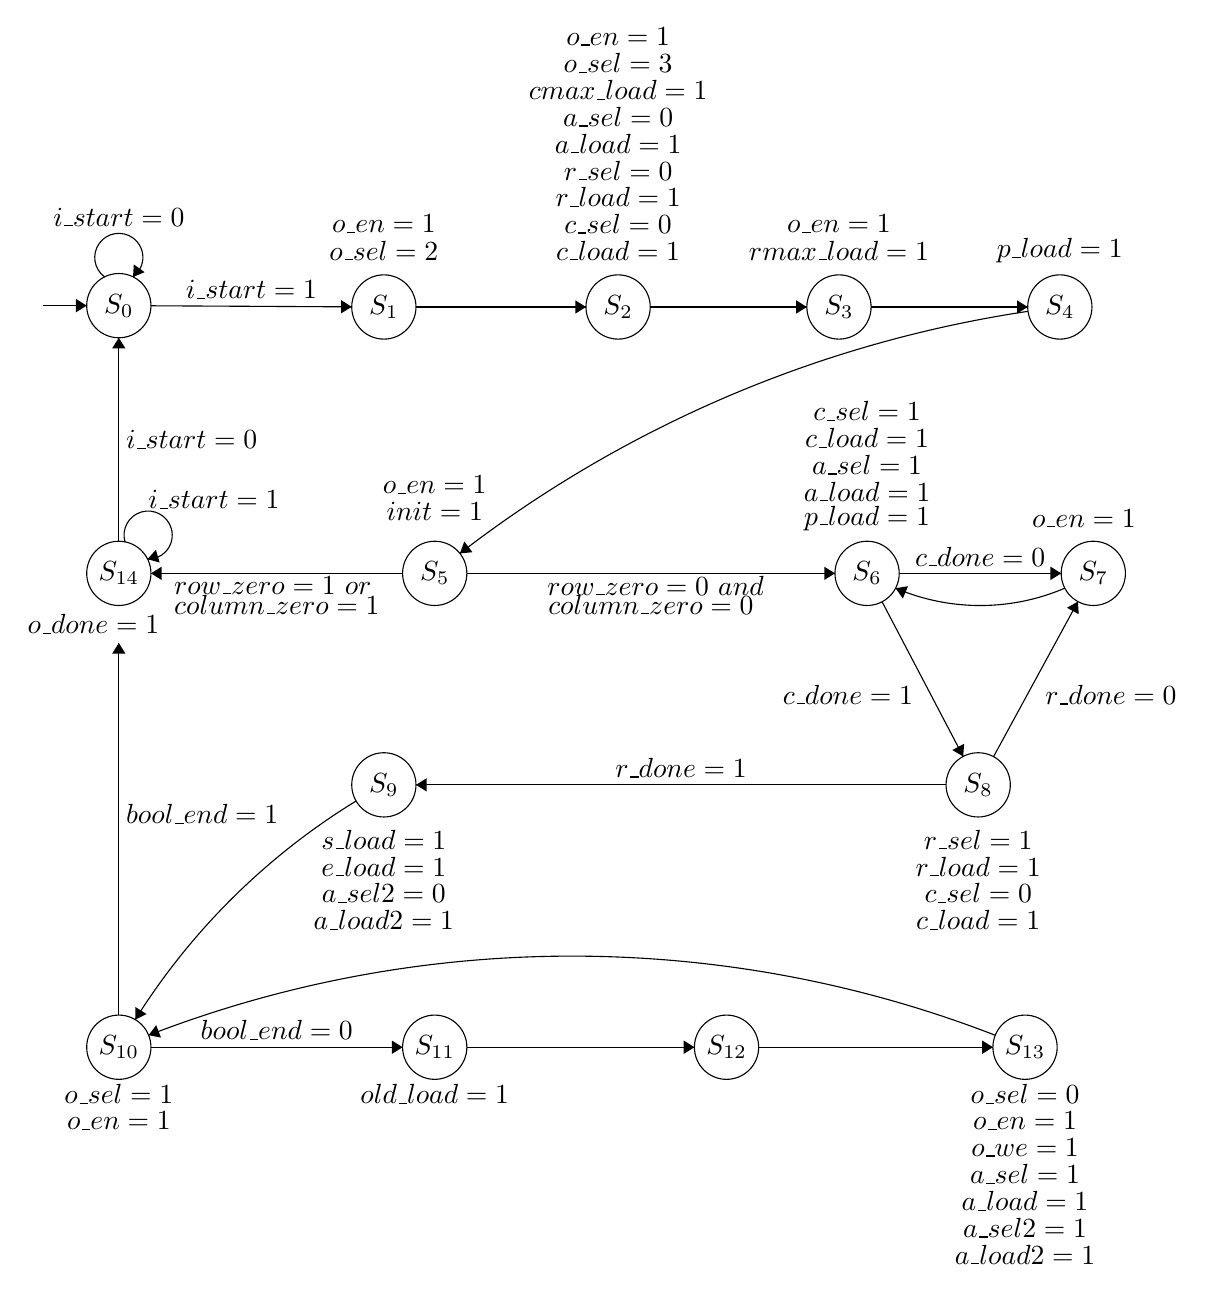
\begin{tikzpicture}[scale=0.17]
\tikzstyle{every node}+=[inner sep=0pt]
\draw [black] (5.9,-5.6) circle (2.4);
\draw (5.9,-5.6) node {$S_0$};
\draw [black] (25.7,-5.7) circle (2.4);
\draw (25.7,-5.7) node {$S_1$};
\draw [black] (43.2,-5.7) circle (2.4);
\draw (43.2,-5.7) node {$S_2$};
\draw [black] (59.7,-5.7) circle (2.4);
\draw (59.7,-5.7) node {$S_3$};
%S1
\draw (25.7,+0.5) node {$o\_en=1$};
\draw (25.7,-1.5) node {$o\_sel=2$};
%S2
\draw (43.2,+14.5) node {$o\_en=1$};
\draw (43.2,+12.5) node {$o\_sel=3$};
\draw (43.2,+10.5) node {$cmax\_load=1$};
\draw (43.2,+8.5) node {$a\_sel=0$};
\draw (43.2,+6.5) node {$a\_load=1$};
\draw (43.2,+4.5) node {$r\_sel=0$};
\draw (43.2,+2.5) node {$r\_load=1$};
\draw (43.2,+0.5) node {$c\_sel=0$};
\draw (43.2,-1.5) node {$c\_load=1$};
%S3
\draw (59.7,+0.5) node {$o\_en=1$};
\draw (59.7,-1.5) node {$rmax\_load=1$};
%S4
\draw (76.2,-1.5) node {$p\_load=1$};
%S5
\draw (29.5,-21) node {$init=1$};
\draw (29.5,-19) node {$o\_en=1$};
%S6
\draw (61.8,-13.5) node {$c\_sel=1$};
\draw (61.8,-15.5) node {$c\_load=1$};
\draw (61.8,-17.5) node {$a\_sel=1$};
\draw (61.8,-19.5) node {$a\_load=1$};
\draw (61.8,-21.5) node {$p\_load=1$};
%S7
\draw (78,-21.5) node {$o\_en=1$};
%S8
\draw (70.1,-45.5) node {$r\_sel=1$};
\draw (70.1,-47.5) node {$r\_load=1$};
\draw (70.1,-49.5) node {$c\_sel=0$};
\draw (70.1,-51.5) node {$c\_load=1$};
%S9
\draw (25.7,-45.5) node {$s\_load=1$};
\draw (25.7,-47.5) node {$e\_load=1$};
\draw (25.7,-49.5) node {$a\_sel2=0$};
\draw (25.7,-51.5) node {$a\_load2=1$};
%S10
\draw (5.9,-64.5) node {$o\_sel=1$};
\draw (5.9,-66.5) node {$o\_en=1$};
%S11
\draw (29.5,-64.5) node {$old\_load=1$};
%S12

%S13
\draw (73.6,-64.5) node {$o\_sel=0$};
\draw (73.6,-66.5) node {$o\_en=1$};
\draw (73.6,-68.5) node {$o\_we=1$};
\draw (73.6,-70.5) node {$a\_sel=1$};
\draw (73.6,-72.5) node {$a\_load=1$};
\draw (73.6,-74.5) node {$a\_sel2=1$};
\draw (73.6,-76.5) node {$a\_load2=1$};
%S14
\draw (4,-29.4) node {$o\_done=1$};

\draw [black] (76.2,-5.7) circle (2.4);
\draw (76.2,-5.7) node {$S_4$};
\draw [black] (29.5,-25.6) circle (2.4);
\draw (29.5,-25.6) node {$S_5$};
\draw [black] (61.8,-25.6) circle (2.4);
\draw (61.8,-25.6) node {$S_6$};
\draw [black] (78.7,-25.6) circle (2.4);
\draw (78.7,-25.6) node {$S_7$};
\draw [black] (70.1,-41.4) circle (2.4);
\draw (70.1,-41.4) node {$S_8$};
\draw [black] (25.7,-41.4) circle (2.4);
\draw (25.7,-41.4) node {$S_9$};
\draw [black] (5.9,-61) circle (2.4);
\draw (5.9,-61) node {$S_{10}$};
\draw [black] (29.5,-61) circle (2.4);
\draw (29.5,-61) node {$S_{11}$};
\draw [black] (51.3,-61) circle (2.4);
\draw (51.3,-61) node {$S_{12}$};
\draw [black] (73.6,-61) circle (2.4);
\draw (73.6,-61) node {$S_{13}$};
\draw [black] (5.9,-25.6) circle (2.4);
\draw (5.9,-25.6) node {$S_{14}$};
\draw (17.4,-26.5) node {$row\_zero=1\mbox{ }or$};
\draw (46,-26.5) node {$row\_zero=0\mbox{ }and$};
\draw [black] (8.3,-5.61) -- (23.3,-5.69);
\fill [black] (23.3,-5.69) -- (22.5,-5.18) -- (22.5,-6.18);
\draw (15.8,-5.13) node [above] {$i\_start=1$};
\draw [black] (0.2,-5.6) -- (3.5,-5.6);
\fill [black] (3.5,-5.6) -- (2.7,-5.1) -- (2.7,-6.1);
\draw [black] (4.842,-3.456) arc (234:-54:1.8);
\draw (5.9,0.3) node [above] {$i\_start=0$};
\fill [black] (6.96,-3.46) -- (7.83,-3.1) -- (7.02,-2.52);
\draw [black] (28.1,-5.7) -- (40.8,-5.7);
\fill [black] (40.8,-5.7) -- (40,-5.2) -- (40,-6.2);
\draw [black] (45.6,-5.7) -- (57.3,-5.7);
\fill [black] (57.3,-5.7) -- (56.5,-5.2) -- (56.5,-6.2);
\draw [black] (62.1,-5.7) -- (73.8,-5.7);
\fill [black] (73.8,-5.7) -- (73,-5.2) -- (73,-6.2);
\draw [black] (31.381,-24.109) arc (127.6527:98.50736:91.678);
\fill [black] (31.38,-24.11) -- (32.32,-24.02) -- (31.71,-23.22);
\draw [black] (31.9,-25.6) -- (59.4,-25.6);
\fill [black] (59.4,-25.6) -- (58.6,-25.1) -- (58.6,-26.1);
\draw (45.65,-28.7) node [above] {$column\_zero=0$};
\draw [black] (27.1,-25.6) -- (8.3,-25.6);
\fill [black] (8.3,-25.6) -- (9.1,-26.1) -- (9.1,-25.1);
\draw (17.7,-28.7) node [above] {$column\_zero=1$};
\draw [black] (64.2,-25.6) -- (76.3,-25.6);
\fill [black] (76.3,-25.6) -- (75.5,-25.1) -- (75.5,-26.1);
\draw (70.25,-25.1) node [above] {$c\_done=0$};
\draw [black] (76.573,-26.706) arc (-66.80792:-113.19208:16.055);
\fill [black] (63.93,-26.71) -- (64.47,-27.48) -- (64.86,-26.56);
\draw [black] (62.92,-27.72) -- (68.98,-39.28);
\fill [black] (68.98,-39.28) -- (69.05,-38.33) -- (68.17,-38.8);
\draw (65.27,-34.65) node [left] {$c\_done=1$};
\draw [black] (71.25,-39.29) -- (77.55,-27.71);
\fill [black] (77.55,-27.71) -- (76.73,-28.17) -- (77.61,-28.65);
\draw (75.07,-34.68) node [right] {$r\_done=0$};
\draw [black] (67.7,-41.4) -- (28.1,-41.4);
\fill [black] (28.1,-41.4) -- (28.9,-41.9) -- (28.9,-40.9);
\draw (47.9,-40.9) node [above] {$r\_done=1$};
\draw [black] (7.126,-58.937) arc (147.92027:121.49805:50.79);
\fill [black] (7.13,-58.94) -- (7.97,-58.52) -- (7.13,-57.99);
\draw [black] (8.3,-61) -- (27.1,-61);
\fill [black] (27.1,-61) -- (26.3,-60.5) -- (26.3,-61.5);
\draw (17.7,-60.5) node [above] {$bool\_end=0$};
\draw [black] (31.9,-61) -- (48.9,-61);
\fill [black] (48.9,-61) -- (48.1,-60.5) -- (48.1,-61.5);
\draw [black] (53.7,-61) -- (71.2,-61);
\fill [black] (71.2,-61) -- (70.4,-60.5) -- (70.4,-61.5);
\draw [black] (8.126,-60.103) arc (111.17339:68.82661:87.555);
\fill [black] (8.13,-60.1) -- (9.05,-60.28) -- (8.69,-59.35);
\draw [black] (5.9,-23.2) -- (5.9,-8);
\fill [black] (5.9,-8) -- (5.4,-8.8) -- (6.4,-8.8);
\draw [black] (5.9,-58.6) -- (5.9,-30.8);
\fill [black] (5.9,-30.8) -- (5.4,-31.6) -- (6.4,-31.6);
\draw (6.4,-43.6) node [right] {$bool\_end=1$};
\draw [black] (6.365,-23.255) arc (196.51907:-91.48093:1.8);
\draw (13,-20.82) node [above] {$i\_start=1$};
\fill [black] (8.04,-24.54) -- (8.95,-24.79) -- (8.67,-23.84);
\draw (6.4,-15.6) node [right] {$i\_start=0$};
\end{tikzpicture}
\end{center}


\section{Risultati Sperimentali}
\subsection{Report di sintesi}
Dal report di sintesi emerge che il modulo è correttamente sintetizzabile e sono stati inferiti 131 Flip Flop e 0 Latch. Il Critical Path limita il clock ad almeno 5.361ns, di conseguenza il constraint di clock imposto da specifica a 100ns è stato rispettato con un ampio margine.
Con un periodo di clock di 15ns, emerge che il tempo massimo di conversione di un'immagine (128x128) risulta essere di 1.48ms.
%Insieme
\subsection{Simulazioni}
Per verificare la correttezza del nostro modulo sono stati utilizzati dei testbench che si ritiene possano stimolare i corner case.\\
I testbench di seguito elencati sono stati utilizzati con lo scopo di verificare il corretto funzionamento del ciclo di lettura della FSM:
\begin{itemize}
    \item Numero di righe e/o numero di colonne uguali a 1.
    \item Immagine di dimensione massima (128x128 pixel).
\end{itemize}
Per testare invece il modulo di calcolo del logaritmo si è scelto di utilizzare i seguenti tesbench:
\begin{itemize}
    \item Immagine bianca (tutti i pixel valgono 255).
    \item Immagine nera (tutti i pixel valgono 0).
    \item Immagine monocromatica (tutti i pixel hanno lo stesso valore).
\end{itemize}
Sebbene un'immagine non possa avere dimensione nulla, per motivi di robustezza, si è scelto di testare comunque questo caso:
\begin{itemize}
    \item Immagini anomale: Numero di righe e/o numero di colonne uguali a 0.
\end{itemize}
Per verificare che l'intero sistema si comporti correttamente nel caso di letture successive e nella gestione dei reset:
\begin{itemize}
    \item Reset sincroni e asincroni durante l'esecuzione.
\end{itemize}
\begin{itemize}
    \item Lettura sequenziale di più immagini.
\end{itemize}
Per verificare che il numero di iterazioni della macchina a stati sia corretto, controllando che anche l'ultimo pixel possa modificare max e min register:
\begin{itemize}
    \item 0 o 255 come ultimo pixel.
\end{itemize}
%Insieme
\section{Conclusioni}
%Insieme

Grazie alle scelte effettuate il sistema risulta particolarmente veloce e scalabile, infatti adottando il modulo Row \& Column counter invece che un moltiplicatore, al crescere delle dimensioni dell'immagine, la complessità temporale aumenta linearmente: con l'utilizzo di un moltiplicatore si andrebbe ad incrementare la durata del clock compromettendo la velocità del circuito.\\




\end{document}
